\documentclass[slidestop]{beamer}
\usetheme{JuanLesPins}
\usepackage{fontenc}

\usepackage[english]{babel}
\usepackage[latin1]{inputenc}
\usepackage{times}
\usepackage[T1]{fontenc}
\usepackage{fontenc}
\usepackage{amssymb}
%\usepackage{pgf,pgfarrows,pgfnodes,pgfautomata,pgfheaps}
\usepackage{amsmath,amssymb}
%\usepackage{tikz}
\usepackage{times}
\usepackage{colortbl}

\usebackgroundtemplate{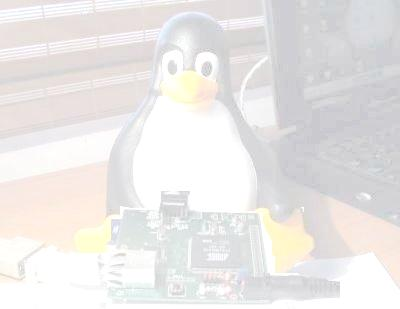
\includegraphics[width=\paperwidth, heigth=\paperheight]{../images/tux_ecb_at91.jpg}}

\title{SIE: Plataforma Rob�tica Para la Ense�anza}
\author{Carlos Iv�n Camargo Bare�o}
\institute[Universidad Nacional de Colombia]{Universidad Nacional de Colombia\\
  Departamento de Ingenier�a El�ctrica y Electr�nica}

\pgfdeclareimage[height=.5cm]{logo}{../images/logo_unal}
\logo{\pgfuseimage{logo}}



\begin{document}

%----------------------------------------------------------------------INSERT TITLE-
\frame[c]{\titlepage}

%$$$$$$$$$$$$$$$$$$$$$$$$$$$$$$$$$$$$$$$$$$$$$$$$$$$$$$$$$$$$$$$$$$$$$$$$$$$$$$$$$$$
%---------------------------------------------------      OPORTUNIDAD    -----------
%$$$$$$$$$$$$$$$$$$$$$$$$$$$$$$$$$$$$$$$$$$$$$$$$$$$$$$$$$$$$$$$$$$$$$$$$$$$$$$$$$$$
\section{Oportunidad}

\subsection{Aprendizaje a trav�s del Dise�o}
% Learning Through Design
% Problem solving can be divided, very roughly, into two categories: analysis and design. Analysis involves decomposing problems into simpler subproblems, typically with the help of formalized rules. Design is different in several ways. In design, the problem goals are typically ill-structured; defining the problem is part of the designer's job. Moreover, there is a somewhat fuzzy sense of what it means to "solve" a design task. Rather than seeking optimal solutions, designers typically seek satisficing solutions [Simon 1969]--that is, solutions that roughly satisfy a given set of constraints.
% 
% 
% Design is important in almost all fields of human activity. Of course, an architect uses design skills when preparing a blueprint. But so does a writer when writing a report, and a manager when restructuring an organization. Given the central role of design in human activity, one would expect design to play an important role in school classrooms. But it doesn't. In the minds of many educators, the ill-structured nature of design activities makes them ill-suited for the classroom. Design activities, they complain, are difficult to "manage" and to evaluate. As a result, students rarely get the opportunity to design, to build, to create, to invent.
% 
% 
% 
% 
% Example 1: Mathematics through design. George, a third-grade student, began his LEGO/Logo work by building a simple LEGO car. First, he connnected the car's motor to a battery box and watched the car roll forward. Next, he connected the motor to the computer and began experimenting with some of the new Logo commands. We explained the commands on, off, onfor (which takes an input and turns on the motor for a designated amount of time), and rd (for reverse direction). After a while, George put several commands together in the following expression: repeat 4 [onfor 20 rd]
% 
% When George executed this expression, the computer turned on the motor for two seconds (onfor 20), reversed the direction of the motor (rd), then repeated those commands three more times. The result: the car moved forward and back, then again forward and back, completing two forward-back cycles.
% 
% Next, George changed the numerical input to repeat. He tried repeat 3 and repeat 6 and repeat 7. After this experimentation, George noticed a pattern:
% 
% When I use an even number, the car ends up where it began. When I use an odd number, it ends up away [from where it started].
% 
% 
% George paused for a moment and then added:
% 
% So that's why there are even and odd numbers!
% 
% Clearly, George had previously learned about even and odd numbers in the classroom. But George's experimentation with the LEGO car provided him with a new (and more personally relevant) representation of the concept. Moreover, the LEGO activity allowed George to relate to numbers in a new way: he played with the ideas of even and odd. This new relationship with even and odd numbers helped George develop a new level of understanding.
% 
% Example 2: Science through design. In some classes, we suggest that students begin their LEGO/Logo work by building motorless "Soap Box Derby" cars. We set up a ramp in the classroom, and students race their cars down the ramp. Some students see a challenge: they want to make their cars go as fast and as far as possible. They measure how far their cars go beyond the bottom of the ramp, then redesign their cars to try to make them go farther.
% 
% As students discuss why some cars go further than others, we encourage students to look for places where "pieces are rubbing together" (for example, gears rubbing against other gears, or axles rubbing against the girders that support them). Before long, discussions about friction become part of the standard discourse between us and the students--and, more importantly, among the students themselves. In one class, a student removed some pieces from his car, explaining (correctly) that "more weight makes things tighter, you know, more friction." Other students give similar explanations. Even after students finish working on their cars and start designing other LEGO/Logo projects, many of them continue to talk about friction in describing and analyzing the motions of their new machines.
% 
% As with even and odd numbers, friction is not a new concept for these students. But the LEGO/Logo activities provide a more meaningful context for students to talk about and think about friction. Students want to make their cars go farther, so friction assumes a new relevance. In short, students care about friction. At first, students' models of friction are rather fragile, and their explanations are often misleading. But as they work on their LEGO/Logo projects (and participate in a "culture" where friction is a standard part of the discourse), students gradually construct richer models of how friction influences the motions of their machines.
% 
% diSessa [1986] describes science learning as a re-experiencing process. Children do not learn a new concept when they are taught the definition. Rather, they must experience and re-experience the concept in different contexts. Through these experiences, children gradually reorganize their intuitions into more complete models. In this case, students, by exploring the motions of LEGO/Logo machines, seem to develop richer and more robust models of friction.
% 
% Learning About Design
% 
% While working on LEGO/Logo design projects, students can learn not only about mathematical and scientific ideas, but about the process of design itself. In particular, students can learn important heuristics, or rules-or-thumb, for dealing with design tasks. Such heuristics are particularly important when working in complex design environments like LEGO/Logo, in which the designer needs to consider several different interrelated design tasks.
% 
% As an example, consider the "vibrating walker" developed by Nicky, a fourth-grade student at a Boston public elementary school. Nicky started by building a car out of LEGO. After racing the car down a ramp several times, Nicky added a motor to the car and connected it to the computer. When he turned on the motor, the car moved forward a bit--but then the motor fell off the body of the car and began vibrating across the table.
% 
% Rather than trying to fix this bug (or giving up since his car had "failed"), Nicky became intrigued with the vibration of the motor. He began to wonder whether he might be able to use the vibrations to power a vehicle. In effect, he decided to turn the vibrations from a bug into a feature.
% 
% 
% 
% Behavior Construction Kits
% 
% 
% 
% During the past few years, a group of us[1] has been working on the development of a new generation of construction kits. Whereas first-generation construction kits allowed children to build structures, and second-generation kits allowed them to build mechanisms, our third-generation kits allow children to build behaviors. Children (and adults too!) have used our new construction kits to build a wide assortment of "behaving machines," such as: a robotic creature that "wants" to move toward the light, a hamster cage that keeps track of the movements of its occupant, and a kinetic sculpture that responds to the movements of a person--or the movements of another machine.
% 
% 
% 
% 
% The Alarm-Clock Bed. John, a fifth-grader at the Hennigan Elementary School in Boston, had an alarm clock next to his bed at home. But the alarm clock wasn't very effective. Often, when the alarm went off, John simply shut off the alarm and went back to sleep. John was determined to invent a better solution. His goal: to design an alarm clock that could not be ignored. John started by playing with the LEGO optosensor. He placed the optosensor by the window, so the computer could "know" when the sun came up. But what should happen at sunrise? John had an idea. He built a small LEGO bed, with a small LEGO person on top. Underneath the bed, he placed a hinged platform, so the bed could tilt from side to side. Alongside the bed, he built a conveyor belt. Then he wrote a Logo program. When the optosensor detected light coming through the window, the program turned on two motors. One motor made the LEGO bed tilt to the side, making the LEGO person slide off onto the conveyor belt. The other motor turned the conveyor belt, carrying the LEGO person out the door. Would John want a full-size version of his alarm-clock ejection bed for his home? Not really, he said. But he certainly enjoyed watching the little LEGO person fly out the door.



  


  % 
  % Imagine
  % Technology needs to provide us with a low floor (an easy way to get started) and a high ceiling (lots of possibilities for taking things even further). There also needs to be wide walls, so that projects can be extended into other domains (from building robots in Lego to building Crickets).
  % 
  % Create
  % The 'Cricket' is a programmable box that can be attached to inanimate objects to make it do things - a cat model that, when stroked, miaows (or when the light sensor is covered, make a noise). These are no pre-programmed toys from Toys R Us that the kid just has and 'interacts' with, but programmable toys that kids can design and develop and truly interact with. What about the characters that start to jump up and down quicker the more  you blow into a sensor? All programmable by the kids.
  % 
  % Play
  % And by taking the physical object we can start to make things happen virtually on a screen, with a free programme like Scratch.
  % 
  % Whole projects can then be designed around invention making, using tools with low floors and limitless ceilings.
  % 
  % Share
  % The one thing Scratch and its website offer us is a way not only to share the products of our learning but also the way we did it, without any extra stages. It would be so good to have a way of doing this in education in general, a way for teachers and students to share the products of their learning and, without too much extra work, the steps they took to get there.
  % 
  % Reflection
  % Going through how you did something, though, is a vital part of reflection and we can only see how we could do things better if we go through this reflective step. I wonder how much reflection is done by Scratchers, though, when it's so easy to upload and then forget about what you have produced. Others, of course, reflect on your work and alter it, but does the payoff not appear mostly for others, rather than the individual who is trying to learn?

% \begin{frame}
%   \frametitle{Sistemas Embebidos: Aplicaciones}
%    \begin{center} 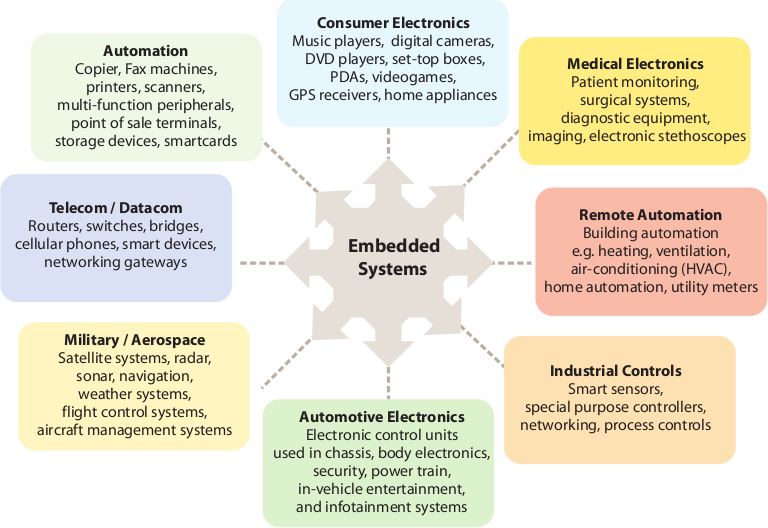
\includegraphics[scale=.5]{../images/Embedded_systems_applications.png}   \end{center}
% \end{frame}
% 
% 
% \subsection[Embedded]{Conocimientos Necesarios}
% \begin{frame}
%   \frametitle{Sistemas Embebidos: Conocimientos Necesarios}
%    \begin{center} 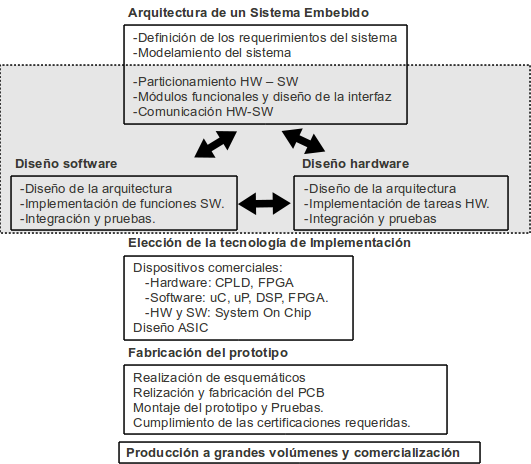
\includegraphics[scale=.51]{../images/ES_CDIO_flow.png}   \end{center}
% \end{frame}



%$$$$$$$$$$$$$$$$$$$$$$$$$$$$$$$$$$$$$$$$$$$$$$$$$$$$$$$$$$$$$$$$$$$$$$$$$$$$$$$$$$$
%----------------------------------------------------------      Clientes          -
\section{Clientes}
%$$$$$$$$$$$$$$$$$$$$$$$$$$$$$$$$$$$$$$$$$$$$$$$$$$$$$$$$$$$$$$$$$$$$$$$$$$$$$$$$$$$


%$$$$$$$$$$$$$$$$$$$$$$$$$$$$$$$$$$$$$$$$$$$$$$$$$$$$$$$$$$$$$$$$$$$$$$$$ $$$$$$$$$$
%----------------------------------------------------------      IMPACTO           -
\section{Impacto}
%$$$$$$$$$$$$$$$$$$$$$$$$$$$$$$$$$$$$$$$$$$$$$$$$$$$$$$$$$$$$$$$$$$$$$$$$$$$$$$$$$$$
 
%$$$$$$$$$$$$$$$$$$$$$$$$$$$$$$$$$$$$$$$$$$$$$$$$$$$$$$$$$$$$$$$$$$$$$$$$$$$$$$$$$$$
%---------------------------------------------------------- MERCADO Y CRECIMIENTO  -
\section{Mercado Y crecimiento}
%$$$$$$$$$$$$$$$$$$$$$$$$$$$$$$$$$$$$$$$$$$$$$$$$$$$$$$$$$$$$$$$$$$$$$$$$$$$$$$$$$$$

%$$$$$$$$$$$$$$$$$$$$$$$$$$$$$$$$$$$$$$$$$$$$$$$$$$$$$$$$$$$$$$$$$$$$$$$$$$$$$$$$$$$
%----------------------------------------------------------   PRODUCTOS/SERVICIOS  -
\section{Productos/Servicios}
%$$$$$$$$$$$$$$$$$$$$$$$$$$$$$$$$$$$$$$$$$$$$$$$$$$$$$$$$$$$$$$$$$$$$$$$$$$$$$$$$$$$

%$$$$$$$$$$$$$$$$$$$$$$$$$$$$$$$$$$$$$$$$$$$$$$$$$$$$$$$$$$$$$$$$$$$$$$$$$$$$$$$$$$$
%----------------------------------------------------------      INVERSION         -
\section{Inversi�n}
%$$$$$$$$$$$$$$$$$$$$$$$$$$$$$$$$$$$$$$$$$$$$$$$$$$$$$$$$$$$$$$$$$$$$$$$$$$$$$$$$$$$

%$$$$$$$$$$$$$$$$$$$$$$$$$$$$$$$$$$$$$$$$$$$$$$$$$$$$$$$$$$$$$$$$$$$$$$$$$$$$$$$$$$$
%----------------------------------------------------------   PR�XIMOS PASOS       -
\section{Pr�ximos Pasos}
%$$$$$$$$$$$$$$$$$$$$$$$$$$$$$$$$$$$$$$$$$$$$$$$$$$$$$$$$$$$$$$$$$$$$$$$$$$$$$$$$$$$

 
 \begin{frame}
   \begin{center}
\includegraphics[scale=.15]{../images/gracias}
   \newline
   \huge{�Gracias!}
   \end{center}
 \end{frame}

\end{document}
